\section{Kinematik}

\textbf{Kinematisches Modell}: Beschreibt Zusammenhänge zwischen \textbf{Gelenkwinkelraum} (Konfigurationsraum) und \textbf{Posenraum des Endeffektors} (Arbeitsraum)

\textbf{Direkte und Inverse Kinematik}:
\begin{itemize}
	\item \textbf{Direkte Kinematik}: 
	\begin{itemize}
		\item Eingabe: Gelenkwinkelstellungen des Roboters
		\item Ausgabe: Pose des Endeffektors
		\item z.B. Wo befindet sich meine Hand?
	\end{itemize}
	\item \textbf{Inverse Kinematik}: 
	\begin{itemize}
		\item Eingabe: Zielpose des Endeffektors
		\item Ausgabe: Gelenkwinkelstellungen
		\item z.B. Wie bewege ich meine Hand zum Ziel?
	\end{itemize}
\end{itemize}
\begin{center}
	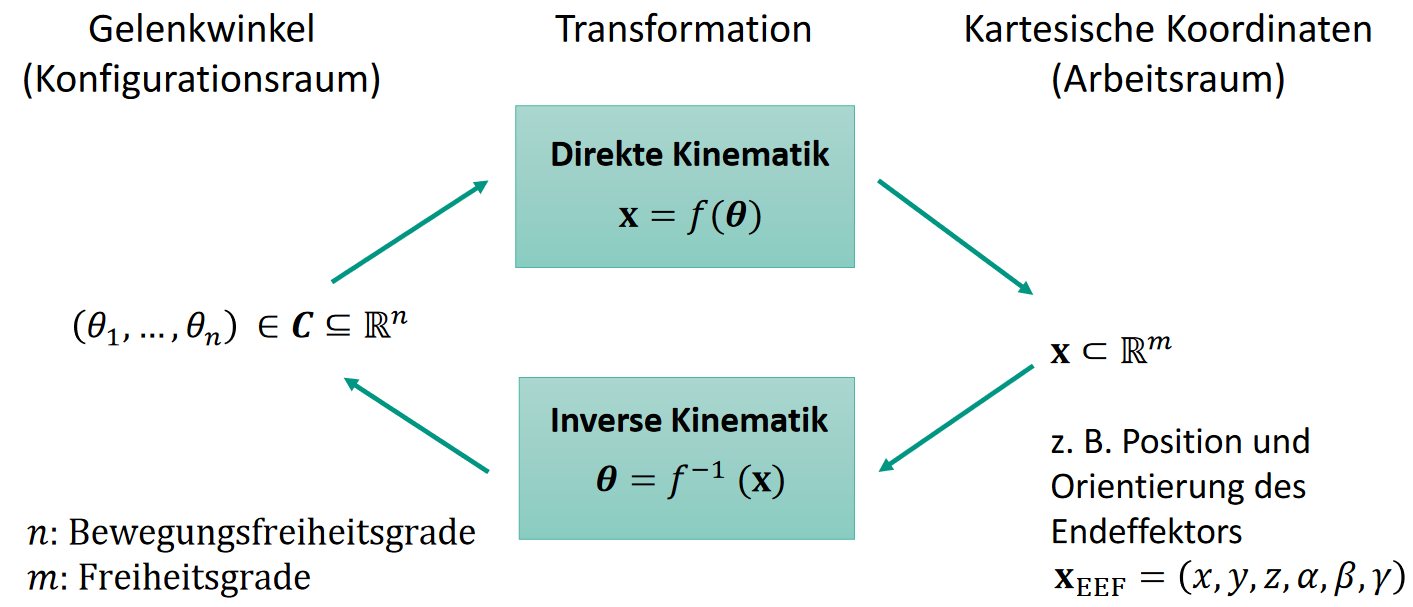
\includegraphics[width=0.7\textwidth]{images/kinematik.png}
\end{center}
\medskip
\textbf{Kinematische Kette} wird von mehreren Körpern gebildet, die durch Gelenke kinematisch verbunden sind (z.B. Roboterarm). Unterscheidung zwischen:
\begin{itemize}
	\item \textbf{Offene} kinematische Kette: Nur ein Ende ist fest, anderes Ende frei bewegbar
	\item \textbf{Geschlossene} kinematische Kette: Beide Enden der Kette sind fest
\end{itemize}
Für jedes Glied müssen \textbf{6 Parameter} für die Transformation zwischen Gelenken bestimmt werden (3 Rotationsparameter, 3 Translationsparameter)
\pagebreak

\textbf{Denavit-Hartenberg (DH) Konvention}:
\begin{itemize}
	\item Durch die geschickte Wahl der Koordinatensysteme lassen sich die Parameter zur Beschreibung eines Armelements auf 4 reduzieren
	\item \textbf{Regeln für Koordinatensysteme}:
	\begin{itemize}
		\item $z_{i-1}$-Achse liegt entlang der Bewegungsachse des $i$-ten Gelenks
		\item $x_i$-Achse verläuft entlang der gemeinsamen Normalen (Kreuzprodukt von $z_{i-1}$ und $z_i$) von $z_{i-1}$ und $z_i$
		\item $y_i$-Achse vervollständigt das Koordinatensystem entsprechend der Rechte-Hand-Regel
	\end{itemize}
	\item \textbf{Parameter des Armelements (DH-Paramerter)}:
	\begin{itemize}
		\item \textbf{Armelementlänge} $a_i$ beschreibt den Abstand von $z_{i-1}$ zu $z_i$ entlang $x_i$
		\item \textbf{Armelementverdrehung} $\alpha_i$ beschreibt den Winkel von $z_{i-1}$ zu $z_i$ um $x_i$
		\item \textbf{Gelenkabstand} $d_i$ ist der Abstand zwischen der $x_{i-1}$-Achse und $x_i$-Achse entlang der $z_{i-1}$-Achse
		\item \textbf{Gelenkwinkel} $\theta_i$ ist der Winkel von $x_{i-1}$ zu $x_i$ um $z_{i-1}$
	\end{itemize}
	\begin{center}
		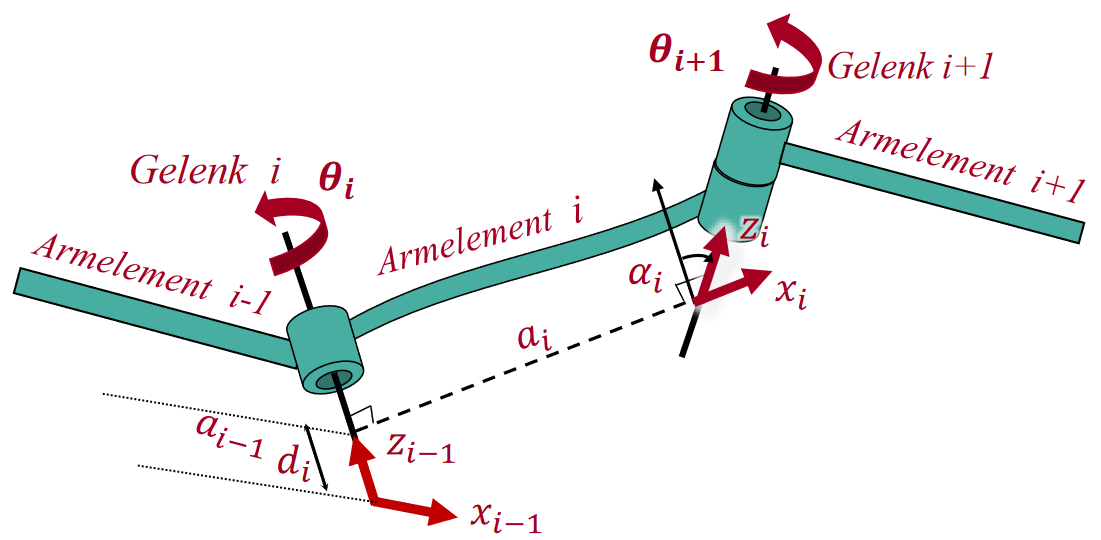
\includegraphics[width=0.7\textwidth]{images/dh.png}
	\end{center}
	\item DH-Parameter beschreiben wie aufeinanderfolgende Gelenke ineinander transformiert werden
	\item \textbf{DH-Transformationsmatrizen}: Beschreibung mit homogenen Matrizen
	\begin{enumerate}
		\item Rotation $\theta_i$: $R_{z_{i-1}}(\theta_i)=\left(\begin{matrix}
			\cos\theta_i & -\sin\theta_i & 0 & 0 \\
			\sin\theta_i & \cos\theta_i & 0 & 0 \\
			0 & 0 & 1 & 0 \\
			0 & 0 & 0 & 1
		\end{matrix}\right)$
		\item Translation $d_i$: $T_{z_{i-1}}(d_i)=\left(\begin{matrix}
			1 & 0 & 0 & 0 \\
			0 & 1 & 0 & 0 \\
			0 & 0 & 1 & d_i \\
			0 & 0 & 0 & 1
		\end{matrix}\right)$
		\item Translation $a_i$: $T_{x_{i}}(a_i)=\left(\begin{matrix}
			1 & 0 & 0 & a_i \\
			0 & 1 & 0 & 0 \\
			0 & 0 & 1 & 0 \\
			0 & 0 & 0 & 1
		\end{matrix}\right)$
		\item Rotation $\alpha_i$:  $R_{x_{i}}(\alpha_i)=\left(\begin{matrix}
			1 & 0 & 0 & 0 \\
			0 & \cos\alpha_i & -\sin\alpha_i & 0 \\
			0 & \sin\alpha_i & \cos\alpha_i & 0 \\
			0 & 0 & 0 & 1
		\end{matrix}\right)$
	\end{enumerate}
	\item Zusammenführen zu einer Matrix:
	\begin{equation*}
	\begin{split}
		A_{i-1,i} &= R_{z_{i-1}}(\theta_i)\cdot T_{z_{i-1}}(d_i)\cdot T_{x_{i}}(a_i)\cdot R_{x_{i}}(\alpha_i) \\
			&= \left(\begin{matrix}
			\cos\theta_i & -\sin\theta_i\cdot\cos\alpha_i & \sin\theta_i\cdot\sin\alpha_i & a_i\cdot\cos\theta_i \\
			\sin\theta_i & \cos\theta_i\cdot\cos\alpha_i & -\cos\theta_i\cdot\sin\alpha_i & a_i\cdot\sin\theta_i \\
			0 & \sin\alpha_i & \cos\alpha_i & d_i \\
			0 & 0 & 0 & 1
		\end{matrix}\right)
	\end{split}
	\end{equation*}
	\item Inverse DH-Transformation:
	\begin{equation*}
		A_{i-1,i}^{-1} = A_{i,i-1} = \left(\begin{matrix}
				\cos\theta_i & \sin\theta_i & 0 & -a_i \\
				-\cos\alpha_i\cdot\sin\theta_i & \cos\theta_i\cdot\cos\alpha_i & \sin\alpha_i & -d_i\cdot\sin\alpha_i \\
				\sin\theta_i\cdot\sin\alpha_i & -\sin\alpha_i\cdot\cos\theta_i & \cos\alpha_i & -d_i\cdot\cos\alpha_i \\
				0 & 0 & 0 & 1
			\end{matrix}\right)
	\end{equation*}
	\item Durch Multiplikation der DH-Matrizen lässt sich die Lage der einzelnen Koordinatensysteme bezüglich des Bezugskoordinatensystems bestimmen
\end{itemize}
\bigskip
\textbf{Direktes kinematisches Problem}: Stellung des Endeffektors (EFF) in Bezug auf das BKS ist gegeben durch: $$S_\text{Basis, EEF}=A_{0,1}(\theta_1)\cdot A_{1,2}(\theta_2)\cdot\cdots\cdot A_{n-2,n-1}(\theta_{n-1})\cdot A_{n-1,n}(\theta_n)$$
Lösung des Problems ergibt sich aus Einsetzen der Gelenkwinkel in obige Gleichung.

\textit{Beispiele 2/38-48}\\

Oft interessiert man sich für verwandte Beziehungen wir z.B. Gelenkwinkelgeschwindigkeiten $\rightarrow$ Endeffektor-Geschwindigkeit. Dafür muss man die Vorwärtskinematik ableiten $\rightarrow$ \textbf{Jacobi-Matrix}
\pagebreak

\textbf{Jacobi-Matrix}: Für eine differenzierbare Funktion $f\colon \R^n\rightarrow\R^m, f(\mathbf{x})=\left(\begin{matrix}
	f_1(\mathbf{x}) \\
	\vdots\\
	f_m(\mathbf{x})
\end{matrix}\right)$ und $\mathbf{x}\in\R^n$ ist die Jacobi-Matrix für ein $\mathbf{a}\in\R^n$ wie folgt:
$$
J_{f}(\mathbf{a})=\left(\begin{array}{ccc}
	\frac{\partial f_{1}}{\partial x_{1}}(\mathbf{a}) & \cdots & \frac{\partial f_{1}}{\partial x_{n}}(\mathbf{a}) \\
	\vdots & \ddots & \vdots \\
	\frac{\partial f_{m}}{\partial x_{1}}(\mathbf{a}) & \cdots & \frac{\partial f_{m}}{\partial x_{n}}(\mathbf{a})
\end{array}\right) \in \mathbb{R}^{m \times n}
$$

\textbf{Problem}: Vorwärtskinematik ist matrixwertig $\rightarrow$ Jacobi-Matrix nicht definiert

\textbf{Lösung}: Vektorwertige Repräsentation wählen, z.B. mit Eulerwinkel\\

\textbf{Geschwindigkeitsraum und Kraftraum}:
\begin{itemize}
	\item Annahme: Kinematische Kette bewege sich entlang einer Trajektorie $\theta\colon\R\rightarrow\R^n$, wobei $\theta$ die Gelenkwinkelstellungen zu einem Zeitpunkt $t$ beschreibt
	\item Pose des End-Effektors $\mathbf{x}(t)\in\R^6$ zum Zeitpunkt $t$: $\mathbf{x}(t)=\mathbf{f}(\boldsymbol{\theta}(t))$, wobei $f$ die Funktion für die Vorwärtskinematik ist
	\item \textbf{Beziehung zwischen Endeffektor- und Gelenkwinkelgeschwindigkeiten}: $$\mathbf{\dot{x}}(t)=J_\mathbf{f}(\boldsymbol{\theta}(t))\cdot\boldsymbol{\dot{\theta}}(t)$$
	\item \textbf{Beziehung zwischen Kräfte und Momente am End-Effektor und Drehmomenten in den Gelenken}:
	$$\boldsymbol{\tau}(t)=J_\mathbf{f}^\top(\boldsymbol{\theta}(t))\cdot\mathbf{F}(t)$$
	wobei $\mathbf{F}\colon\R\rightarrow\R^6$ der Kraft-Momenten-Vektor am End-Effektor und $\boldsymbol{\tau}\colon\R\rightarrow\R^n$ die Drehmomente in Gelenken ist
	\item Im Geschwindigkeits- und Kraftraum lässt sich die Frage nach der Inversen Kinematik durch die Inverse der Jacobi-Matrix lösen, z.B. Welche Gelenkwinkelgeschwindigkeiten sind notwendig, um eine End-Effektor-Geschwindigkeit zu realisieren? $\rightarrow$ Löse nach $\boldsymbol{\dot{\theta}}(t)$ auf
\end{itemize}
\bigskip
\textbf{Berechnung der Jacobi-Matrix}:
\begin{itemize}
	\item Jede Spalte der Jacobi-Matrix gehört zum Gelenk $\theta_i$ der kinematischen Kette
	\item Wenn $j$-tes Gelenk ein Translationsgelenk ist, das eine Translation in Richtung des Einheitsvektors $\mathbf{z_j}\in\R^3$ durchführt, gilt für die $j$-te Spalte der Jacobi-Matrix:
	$$J_j(\boldsymbol{\theta})=\left[\begin{matrix}
		\mathbf{z_j} \\
		\mathbf{0}
	\end{matrix}\right]\in\R^6$$
	\item Wenn $j$-tes Gelenk ein Rotationsgelenk ist, das eine Rotation um die Rotationsachse $\mathbf{z_j}\in\R^3$ an der Position $\mathbf{p_j}\in\R^3$ durchführt, gilt für $j$-te Spalte der Jacobi-Matrix:
	$$J_j(\boldsymbol{\theta})=\left[\begin{matrix}
		\mathbf{z_j}\times(\mathbf{f}(\boldsymbol{\theta})-\mathbf{p_j}) \\
		\mathbf{z_j}
	\end{matrix}\right]\in\R^6$$
\end{itemize}

\textit{Beispiel 2/68-72}\\

\textbf{Kinematische Singularitäten}:
\begin{itemize}
	\item \textbf{Definition}: Wenn sich Roboter in einer Konfiguration $\boldsymbol{\theta}_\text{singular}\in C$ befindet, in der er sich nicht instantan in eine oder mehr Richtungen bewegen kann
	\item Bedeutet, dass Jacobi-Matrix $J(\boldsymbol{\theta})$ keinen vollen Rang bzw. min. zwei linear abhängige Spalten hat, also nicht invertierbar ist
	\begin{center}
		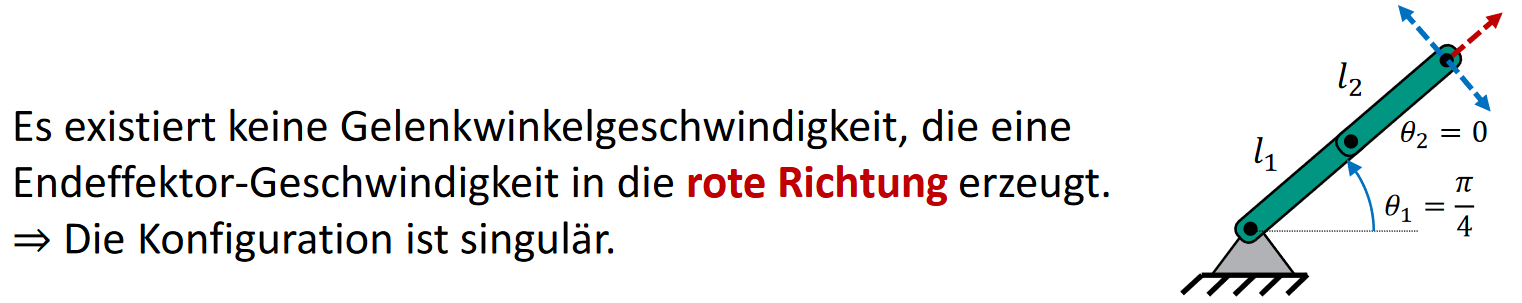
\includegraphics[width=0.7\textwidth]{images/singular.png}
	\end{center}
\end{itemize}
\bigskip
\textbf{Manipulierbarkeit}: Maß für die Bewegungsfreiheit des Endeffektors, bzw. wie nahe eine Konfiguration an einer Singularität ist
\begin{itemize}
	\item Nutze $J(\boldsymbol{\theta})$ um Einheitskreis der Gelenkwinkel-Geschwindigkeiten in den Raum der Endeffektor-Geschwindigkeiten abzubilden 
	
	$\rightarrow$ Resultat: \textbf{Ellipsoid der Manipulierbarkeit}
	
	\item Kreis: Bewegungen des Endeffektors in alle Richtungen uneingeschränkt möglich
	\item Degenerierte Fälle (gestauchtes Ellipsoid): Endeffektor-Bewegung ist in bestimmen Richtungen eingeschränkt
	\begin{center}
		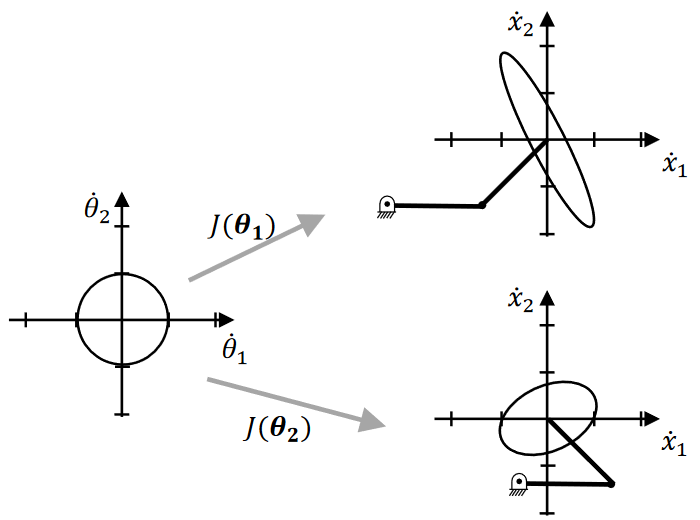
\includegraphics[width=0.5\textwidth]{images/edm.png}
	\end{center}
	\newpage
	
	\item Singulärwerte von $J(\boldsymbol{\theta})$ sind die Wurzeln der Eigenwerte von $J(\boldsymbol{\theta})\cdot J(\boldsymbol{\theta})^\top$, also $\sigma_i=\sqrt{\lambda_i}$, wobei $\lambda_i$ ein EW von $J(\boldsymbol{\theta})\cdot J(\boldsymbol{\theta})^\top$ ist
	\item \textbf{Skalare Maße} für die Manipulierbarkeit:
	\begin{itemize}
		\item Kleinster Singulärwert $\mu_1(\boldsymbol{\theta})=\sigma_\text{min} (A(\boldsymbol{\theta}))$
		\item Inverse Kondition: $\mu_2(\boldsymbol{\theta})=\cfrac{\sigma_\text{min} (A(\boldsymbol{\theta}))}{\sigma_\text{max} (A(\boldsymbol{\theta}))}$
		\item Determinante: $\mu_3(\boldsymbol{\theta})=\det A(\boldsymbol{\theta})$
	\end{itemize}
	\item \textbf{Kraft-Ellipsoid}: Selbiges kann man auch für den Kraftraum einführen
	\begin{center}
		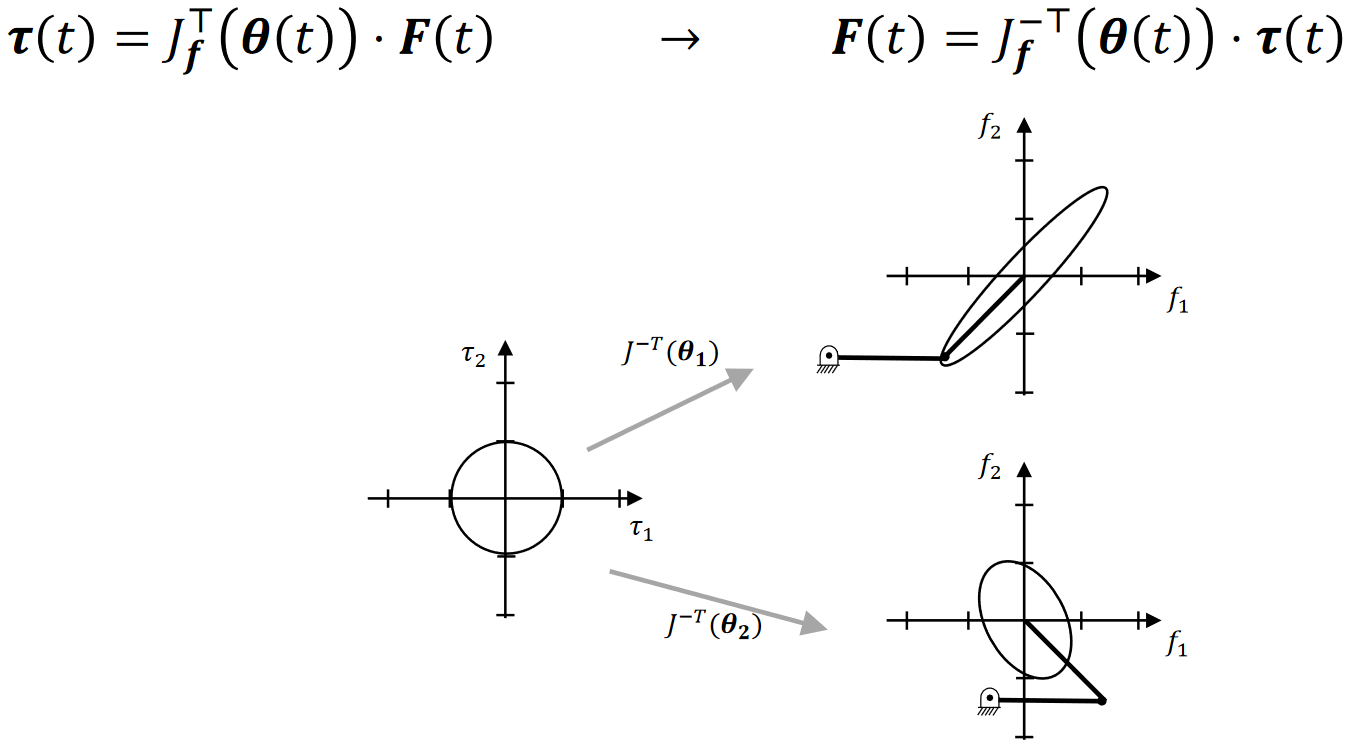
\includegraphics[width=0.7\textwidth]{images/kraft-ellipsoid.png}
	\end{center}
\end{itemize}
\bigskip
\textbf{Geometrisches Modell}:
\begin{itemize}
	\item \textbf{Einsatzbereiche}: 
	\begin{itemize}
		\item Abstandsmessung und Kollisionserkennung
		\item Graphische Darstellung von Körpern
		\item Berechnung der Bewegungen von Körpern
		\item Ermittlung der wirkenden Kräfte und Momente
	\end{itemize}
	\item \textbf{Klassifizierung} nach \textbf{Raum} (2D oder 3D) oder \textbf{Grundprimitiven} (Kanten- bzw. Drahtmodelle, Flächen- bzw. Oberflächenmodelle, Volumenmodell)
\end{itemize}
